\documentclass{article}
\usepackage[UTF8]{ctex}
\usepackage{geometry}
%\usepackage{natbib}
\usepackage{graphicx}
\usepackage{setspace}
\usepackage{caption2}
\usepackage{datetime}
\usepackage{float}

\pagestyle{plain}
\geometry{left=3.18cm,right=3.18cm,top=2.54cm,bottom=2.54cm}

\setmainfont{Times New Roman}
\setCJKmainfont{黑体}

\renewcommand{\today}{\number\year 年 \number\month 月 \number\day 日}
\renewcommand{\captionlabelfont}{\small}
\renewcommand{\captionfont}{\small}

\begin{document}

\begin{figure}
    \centering
    
\includegraphics[width=8cm]{upc.png}
    \label{figupc}
\end{figure}

\begin{center}
	\quad \\
	\quad \\
	\heiti \fontsize{45}{17} \quad \quad \quad
	\vskip 1.5cm
	\heiti \zihao{2} 《计算科学导论》课程总结报告
\end{center}

\vskip 2.0cm
	
\begin{quotation}
	\doublespacing
    \zihao{4}\par\setlength\parindent{7em}
	\quad

	学生姓名:\underline{\quad \qquad \ 张森 \ \qquad \quad}

	学\hspace{0.6cm} 号:\underline{\qquad \ 1907010114 \ \qquad}
		
	专业班级:\underline{\qquad \ 计算1901 \ \qquad  }
		
    学\hspace{0.6cm} 院:\underline{计算机科学与技术学院}

	\vskip 2cm
	\centering
	\begin{table}[h]
        \centering
        \zihao{4}
        \begin{tabular}{|c|c|c|c|c|c|c|}
            \hline
            课程认识 & 问题思 考 & 格式规范  & IT工具  & Latex附加  & 总分 & 评阅教师 \\
            30\% & 30\% & 20\% & 20\% & 10\% &  &  \\
            \hline
             & & & & & &\\
             & & & & & &\\
            \hline
        \end{tabular}
    \end{table}
	\vskip 2cm
	\today
\end{quotation}

\thispagestyle{empty}
\newpage

\setcounter{page}{1}

\section{引言}

计算科学导论这门课程,作为计算机科学与技术专业的学科思政课程,从计算科学的历史渊源、学科特点、学科知识体系结构、学科发展规律和趋势等内容,引导学生从科学哲学的角度去认识和学习计算科学,帮助学生更好的认识本科培养方案及培养目标,助力学生建立起对学校“努力构建面向产出的、质量可控的、量化的人才培养体系”的科学合理的认识与分析,使得学生向着成为社会主义合格的建设者和接班人的目标不忘初心,砥砺奋斗。

作为一名计算机科学与技术专业的大一新生,我很荣幸能够听到孙运雷教授为我们带来别开生面的计算科学导论课程。孙教授为我们开启了计算科学的大门,带领我们遨游在计算科学的海洋中,不仅帮助我们拓宽计算科学的视野,而且还帮助我们构建起合理的课程先修关系图及软件研发、网络规划、系统架构、智能应用四个方面的支撑课程。借此机会,请允许我代表计算机科学与技术专业2019级全体同学,向孙教授致以由衷的感谢与最崇高的敬意!

本文将结合我在计算科学领域的学习经历、认识体会等方面,结合课程中对分组演讲DDoS的探索,对其他网络安全相关领域的认知,分析总结计算科学导论这门课程的重要性及这一阶段的所思所感。希望对自己后续的学习、科研方面起到启蒙的作用,成为后续不懈奋斗的力量源泉。

\section{对计算科学导论这门课程的认识、体会}
任何一门学科都有其独特的科学。

基于计算机学科的计算科学,通过对逻辑结构和经验内容的分析,对科学理论和客观世界关系的分析,对科学理论和科学家关系的分析,帮助我们逐步建立起计算科学的学科方法论和学科方法学。而我国高等院校建设的核心目标就是致力于人才素质的综合培养,对所学专业进行系统化、规范化的建设,使其具有可塑造性和建设性。

计算科学导论这门课程便是如此,它带领大一新生从对计算科学的懵懂到了解,从迷茫到坚定,更加清晰地认识到了当下计算科学发展之机遇,确定自己的目标,追求人生价值的实现。
本节将结合半年来计算科学的学习经验与体会,浅谈计算科学、计算思维和计算人才培养三个方面进行阐述,以彰显计算科学导论这门课程对我在计算科学领域方面的影响,体现计算科学导论对于大一新生的重要性。

\subsection{浅谈计算科学}

计算科学是对描述和变换信息的算法过程,包括其理论、分析、设计、效率分析、实现和应用的系统,是一种新的科学形态。

狭义上,计算科学指的是计算机科学与技术这一一级学科,而广义上,还囊括了计算作为一个学科形态所包含的学术范畴和内涵。自然,研究计算科学,要先研究科学的认识论、科学方法论和科学的逻辑基础。一个科学的认识,一套科学的方法,一套科学的程序,便可以帮助我们探究计算科学哲学,了解计算科学与其他学科的联系,理解计算科学的学科形态、核心概念、典型方法和典型实例。

以数学和电子科学为基础,计算科学是一门理论性、实践性很强的新兴学科,但目前整体上对计算科学的理论研究仍然滞后于技术开发。举例来说,当下对于芯片制造行业来说,深究5nm工艺背后的理论支持或许并不那么容易,但是参照经验科学的工作方式却可能将其规模量产。计算科学并不完全排斥经验科学,但是单纯靠经验科学来发展一门学科,是极其不稳定的。

社会的广泛应用需求推动了计算科学的发展,新一代信息技术产业大都与计算科学的发展密切相关。5G、新型电子元器件、集成电路设计制造……计算科学正帮助人类突破一道又一道技术难关,更好的服务于社会,贡献于世界。

\subsection{浅谈计算思维}

计算思维是一种重要的思维方式\cite{ref1}。它最早由麻省理工学院的Seymour Papert教授提出\cite{ref2},并由卡内基梅隆大学的周以真教授推广\cite{ref3}。对于计算思维的理解和应用,具有极为重要的意义。

计算思维能够帮助我们将一个具体的问题抽象化,进而形成能让计算机“理解”的可计算模型,并且在有限的时空内得出结果。它在专业能力和信息素质培养上的重要性是不言而喻的。它不仅是把现实问题变成计算机可计算模型并产生结果的思维过程,而且它与计算实践密切相关。

众所周知,计算科学拥有着悠久的数学起源。从丢番图方程到可计算性问题,一次又一次数学危机引导人们不断探索计算科学之哲学思想。哥德尔的不完备定理的出现,使得许多数学家试图将可计算性理论形式化,一般递归函数、λ算子、图灵机便是其中典型的代表。而随着计算科学的发展,计算思维也随之形成。

随着计算机智能化程度的提升和计算能力的不断增强,人类对于世间万物的认知,对于复杂算术的运算,对于抽象问题的解决,都是人类计算思维的综合体现。伴随着计算实践,计算思维才能服务于设计和构造,才能帮助人们认识、研究和改造世界,进而促进社会的进步。

因此,没有计算实践而空谈计算思维是没有意义的,我们自然而然也无法感觉到程序的美感。当然,无论我们未来是否从事与计算科学相关的工作,这种将一个大问题分解为若干个子问题的自顶向下的结构化设计方法会充斥在我们的日常生活中,帮助我们处理生活的琐事,更加清晰的认识世界和改变世界。

\subsection{浅谈计算人才培养}

近年来,中美贸易摩擦的不断升级和美国在芯片产业上对中国的封锁,极大的震撼了中国的产业界,这也为计算人才的培养敲响了警钟。

《教育部关于深化本科教育教学改革全面提高人才培养质量的意见》\cite{ref4}指出,要进一步指定个性化的培养方案和学业生涯规划,推进模块化课程建设,丰富优质课程资源,进一步激励学生刻苦学习,引导学生爱国、励志、求真、力行。

我校计算机科学系“努力构建面向产出的、质量可控的、量化的人才培养体系” \cite{ref5},帮助国家培养适应新时代信息化、网络化、智能化深度驱动社会主义现代化发展需要,能够在计算应用及相关领域从事软件研发、网络规划、系统架构或智能应用等工作的工程技术人才。

在现行的2019版培养方案中,学校设立13项毕业要求,36条毕业要求指标点,帮助学生培养问题分析、分析开发方案、研究与设计等能力,不仅帮助学生培养了计算思维,培养了基本的技能,而且鼓励学生的个性化发展,在四个发展方向上开拓思维,锻炼能力,提升学生的综合素质和专项能力。

我相信,在共和国纲领性文件的指导下,在学校的培养下,在计算机科学系老师们辛勤的付出下,越来越多的计算人才将不断涌现,终为我国培养出德智体美劳全面发展的社会主义建设者和接班人。

\section{进一步的思考}

\subsection{DDoS的基本概念与基本知识}

纵观全球,随着互联网、物联网的发展,DDoS的攻击成本越来越低,攻击逐渐趋于平台化和服务化。同时,在许多行业内存在激烈的竞争,恶性竞争的行业往往通过低成本的网络攻击获取更大利益,DDoS自然而然成为了不错的选择。

而且,随着IPv6及5G的进一步普及,IoT网络的迅猛发展致使海量的IoT终端面临加入“僵尸军团”的极大风险,促使攻击成本进一步降低,且越来越多的反射源被挖掘出来,导致攻击带宽不断增大。且随着DDoS攻击日趋复杂化,传统防御技术遭受到越来越严峻的挑战。

本节将就DDoS的攻防陈述个人观点,并通过相关资料及书籍预测DDoS新型防御技术的发展前景和未来预期。

\subsubsection{DDoS的基本知识}

通过对书籍《破坏之王:DDoS攻击与防范深度剖析》\cite{ref6}的阅读,我了解到分布式拒绝服务攻击(Distributed Denial of Service,DDoS),是一种分布式、协作式、大规模的利用若干台机器同时向一个或多个目标发动网络攻击的攻击方式。

\subsubsection{传统DDoS的攻击方式}

DDoS逐渐趋于工具化、武器化、普及化。它是谋取利益强有力的工具,是网络战最锋利的武器,并且DDoS的相关工具也逐渐变得简易化、高效化。

传统的DDoS攻击方式主要利用攻击网络带宽资源、系统资源、应用资源三种途径进行分布式拒绝服务攻击。利用网络带宽资源攻击,即攻击者利用大量数据包消耗攻击目标的带宽资源,使得其余正常请求无法得到及时、有效的响应,造成拒绝服务;利用系统资源攻击,即攻击者消耗和占用系统连接资源,阻碍正常连接与服务器建立会话,造成拒绝服务;利用应用资源攻击,即攻击者提交大量消耗资源的请求时,应用服务无法应对如此巨大的资源消耗,便无法为正常用户提供服务,造成拒绝服务。

当然,攻击者还会对上述三种方式综合运用,以造成危害更大的攻击效果,从而达成其攻击意图。

\subsubsection{传统DDoS的防御方式}

对于DDoS的防御,主要包含两大部分——对攻击流量的稀释和清洗。

稀释,便是对攻击流量的淡化处理,其方法之一便是负载均衡。就好比将高浓度的糖水加入到大海中一样,通过内容分发网络(CDN)达到负载均衡的效果,在互联网中设置多个节点作为代理缓存,使得攻击流量分散到对应的CDN节点上,达到流量稀释的效果。不过,CDN技术仅通过对域名发起的攻击有稀释作用,若直接通过IP地址攻击服务器,则无法稀释攻击流量。

清洗,便是对攻击流量的分类处理,其方法之一便是信誉检查。就好比社会上的征信系统一样,通过对每个请求的IP地址根据请求的特征及其历史记录设置一个信誉值,而为请求设置优先级。优先处理优先级较高的请求而丢弃较低的请求,从而达到对DDoS攻击流量的分类,进而屏蔽这部分流量。不过,由于攻击者可采用动态IP,且若设置IP黑名单容易导致误报现象,清洗的难度较高。

对攻击流量的稀释与清洗联合应用,可提升对DDoS的防御效果。此外,提高服务器处理能力,增大网络带宽也不失为一种选择。可见,DDoS的防御成本是相当高的,这也是通过DDoS攻击进行勒索的一大原因。

\subsubsection{新型DDoS的攻击方式}

未来,DDoS攻击将逐渐出现更为高级、更加高效的攻击技术,其持续时间将会随着攻击策略的调整有所增加,所造成的危害将会越来越严重。

基于上述认识,我学习了IEEE论文\emph{Temporal lensing and its application in pulsing denial-of-service attacks}\cite{ref7},介绍了一种新型的DDoS的攻击方式——脉冲波。

攻击者通过单台主机,利用不同线路的传输时间的时间差,使得多份信息同时到达目标服务器,这就是脉冲波的主要思想。

\begin{figure}[h!]
    \centering
    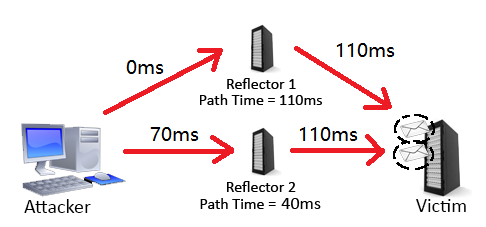
\includegraphics[scale=0.6]{1}
    \caption{脉冲波攻击示意图}
    \label{fig:1}
\end{figure}

不难设想,倘若攻击者利用僵尸网络同时对目标服务器发动脉冲波攻击,则会造成更加严重的危害。

2017年起,活跃的僵尸网络便利用此技术发动DDoS攻击。相较于原有的攻击技术,脉冲波攻击有能力在几秒钟内调动一个攻击峰值高达350Gbps 的攻击流量,远高于正常DDoS攻击的1Gbps的攻击峰值。短暂快速的攻击使得基于被DDoS流量淹没的被动防御缺乏足够的时间和带宽触发提供的防护与缓解措施。

可见,运用此类攻击方式的攻击者对攻击资源具有极高的掌控能力,同时该类攻击也具有成熟且强大的僵尸网络的支持。

\subsubsection{新型DDoS的防御方式}

了解到新型攻击方式之后,我又学习了IEEE论文\emph{A Honeypot with Machine Learning based Detection Framework for defending IoT based Botnet DDoS Attacks}\cite{ref8}。

首先,我了解了蜜罐技术。它本质上是对攻击者的一种欺骗方式,通过布置主机、散布信息、网络服务诱使攻击者对“蜜罐”进行攻击,进而捕获攻击者的信息和行为模式,了解攻击者的攻击工具和攻击方式,推测攻击者的攻击意图,最终提升系统的整体安全防护能力。

\begin{figure}[h!]
    \centering
    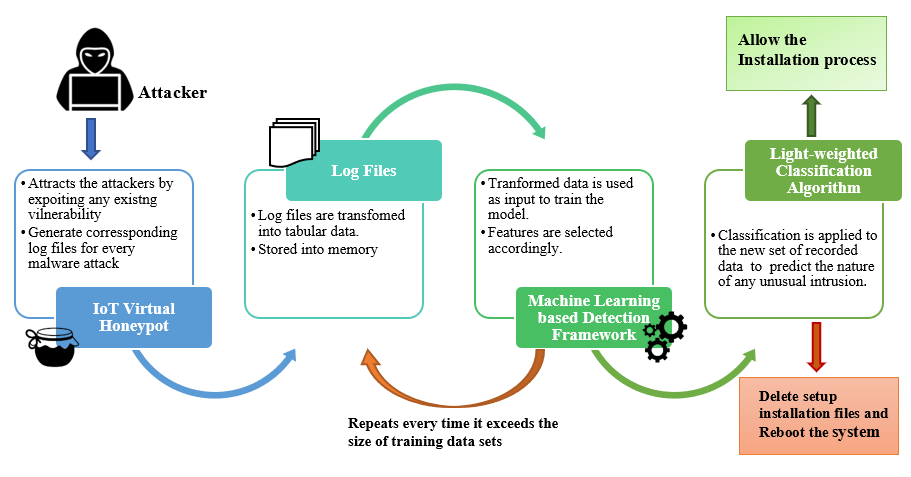
\includegraphics[scale=0.6]{2}
    \caption{基于结合机器学习的蜜罐技术的对使用物联网设备进行DDoS攻击的检测框架流程图}
    \label{fig:2}
\end{figure}

基于结合机器学习的蜜罐技术对使用物联网设备进行DDoS攻击的检测框架主要通过蜜罐技术,诱导对物联网设备进行攻击,通过机器学习的方式对攻击者及僵尸网络的攻击行为进行特征捕捉,并对系统防御方式进行有针对性地优化,以便预测可能的非正常访问,从而大大提高DDoS的治理和缓解能力。

\subsection{2019年DDoS攻击态势}

为了了解2019年的DDoS的攻击态势,我查阅了由中国电信和绿盟科技发布的《2019年DDoS攻击态势》报告\cite{ref9}。

\begin{figure}[h!]
    \centering
    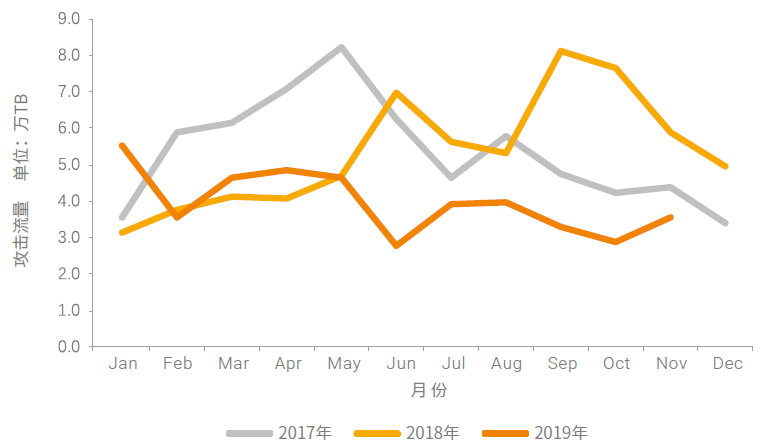
\includegraphics[scale=0.6]{3}
    \caption{近三年所监控到的DDoS攻击流量}
    \label{fig:3}
\end{figure}

2019年,DDoS攻击平均峰值与2018年相比稳中有升,大规模攻击技术的成熟度逐年提升。一方面,攻击者不局限于单一的DDoS攻击,而选择与勒索软件、挖矿木马等合作攻击,来最大化自身利益。另一方面,物联网设备的DDoS参与度逐年提升,因IoT设备数量多,在线时间长,漏洞较多,容易被攻击者所利用,需要有关企业和部门进一步加强感知、预防和治理。

DDoS这种古老的攻击方式,简单、直接、有效。DDoS防护不再依赖设备和检测算法的堆积,更需要安全生态合作和协同防护。漏洞挖掘与披露,网络测量与感知,威胁狩猎与情报共享,防御资源调度与应急响应,随着大规模攻击组织能力的提升,安全厂商和运营商也需要更好的协同。在做好技术层面的防护和跟踪同时,更要做好活力渠道和攻击动机的监控。

\subsection{对于DDoS的个人思考}

谈及DDoS,似乎离我们的日常生活很远很远,殊不知,在每一天都有数不尽的DDoS攻击发生。它们或用于商业竞争,成为企业间竞争的工具;它们或用于军事作战,成为国家间信息化实力比拼的武器;它们或用于表达政治观点,通过工具进行“无声的抗议”;它们或用于谋取个人利益,通过勒索进行非法敛财。

DDoS防御的成本往往要远高于攻击的成本。攻击只需要租用甚至入侵一些主机,建立起“僵尸网络”,运用一定的攻击策略,对目标服务器进行攻击。而防御,则需要花费大量资金提升服务器配置以应对大量请求,增大带宽以防止带宽被非法流量全部占据,研究算法以动态平衡攻击流量减轻服务器压力。

DDoS在可预见的未来,仍然会是网络攻击的主要攻击方式,仍然会是攻击成本远远低于防御成本的利剑。我们期待着,在机器学习和人工智能的进一步发展,利用逆向追踪等技术,通过AI动态分析攻击流量的特点,进而分析出攻击者的地址或攻击行为模式,从根源上解决每一次DDoS攻击,或许会是降低其防御成本的一项方法。

DDoS防御,任重而道远,而吾将上下而求索,积极实践在网络安全领域,或许未来的某一天,能对低廉的DDoS防御尽自己的一份力量。


\section{总结}

时光荏苒,岁月如梭,半年大学生活转瞬即逝。在孙运雷教授的指导下,我了解到了计算科学的发展历程,认识到了计算科学未来的发展方向,学习到了DDoS的相关知识,感受到了计算科学导论这门课程的重要性。

我知道,计算科学导论只是引导我们去了解计算科学下的诸多分支,帮助我们浅显的认识分支学科所包含的内容及其未来可能的发展方向,帮助我们更好的度过大一迷茫的生活,桥接高中与大学,帮助我们更清晰的认识到计算科学发展现状,引导我们认识问题、思考问题,尝试给出可能的解决方案,锻炼我们的基本素质。

未来,我将不负韶华,以更加饱满的精力,更加坚定的决心,更加顽强的毅力,更加努力的探索,在计算科学导论所建成的总体框架下,不忘初心,认真学习科学文化知识,全面提高自身综合素质,向着成为一名网络安全方面人才不断前行,向着成为社会主义事业合格的建设者和接班人不懈奋斗。

\section{附录}

\subsection{Github}

个人网址:https://github.com/Johnsonsky

截图:
\begin{figure}[H]
    \centering
    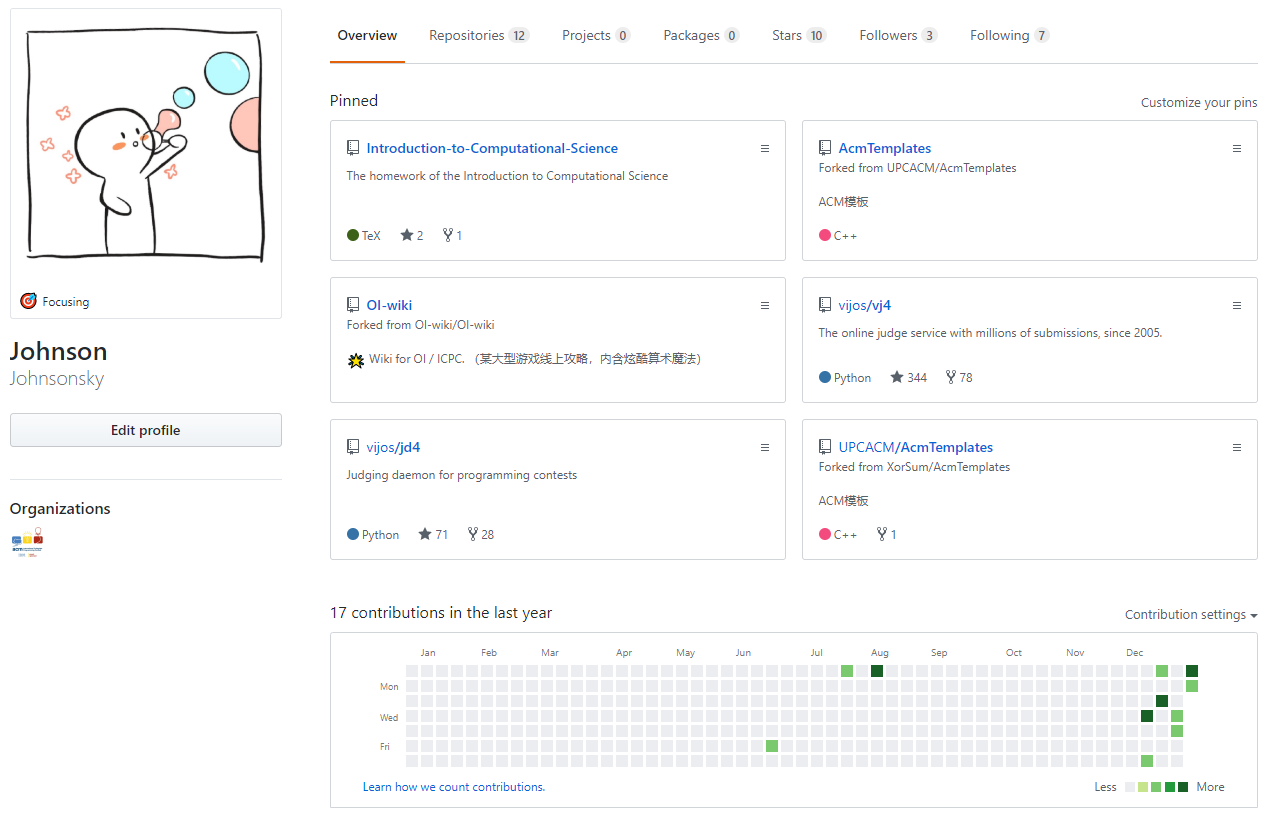
\includegraphics[scale=0.3]{F1}
    \label{fig:F1}
\end{figure}

\subsection{观察者}

截图:
\begin{figure}[H]
    \centering
    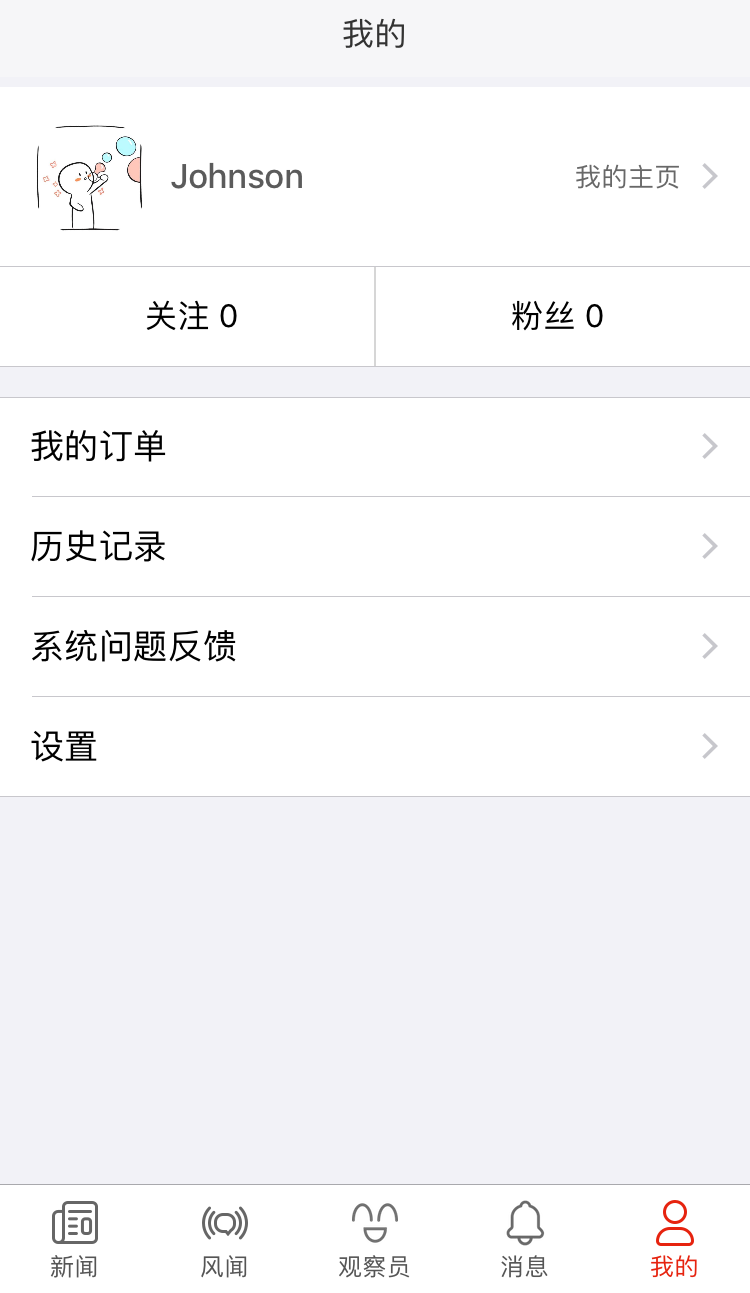
\includegraphics[scale=0.28]{F2}
    \label{fig:F2}
\end{figure}

\subsection{学习强国}

截图:
\begin{figure}[H]
    \centering
    
\includegraphics[scale=0.28]{F3}
    \label{fig:F3}
\end{figure}

\subsection{哔哩哔哩}

截图:
\begin{figure}[H]
    \centering
    
\includegraphics[scale=0.28]{F4}
    \label{fig:F4}
\end{figure}

\subsection{CSDN}

个人网址:https://blog.csdn.net/qq\_21176885

截图:
\begin{figure}[H]
    \centering
    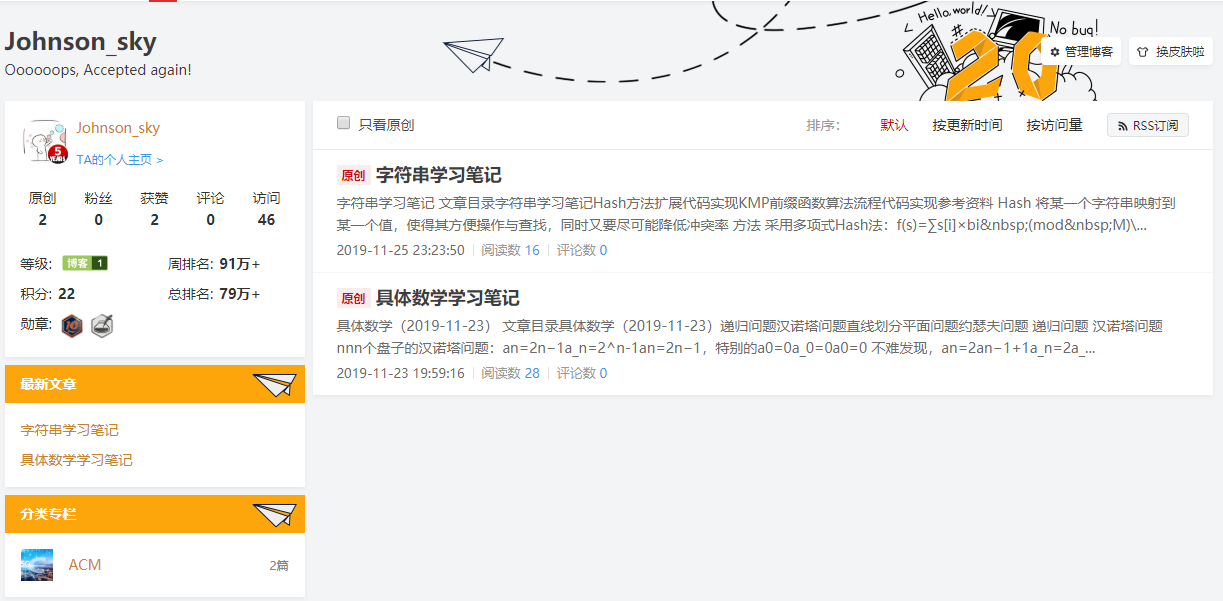
\includegraphics[scale=0.5]{F5}
    \label{fig:F5}
\end{figure}

\subsection{博客园}

个人网址:https://www.cnblogs.com/johnson0130/

截图:
\begin{figure}[H]
    \centering
    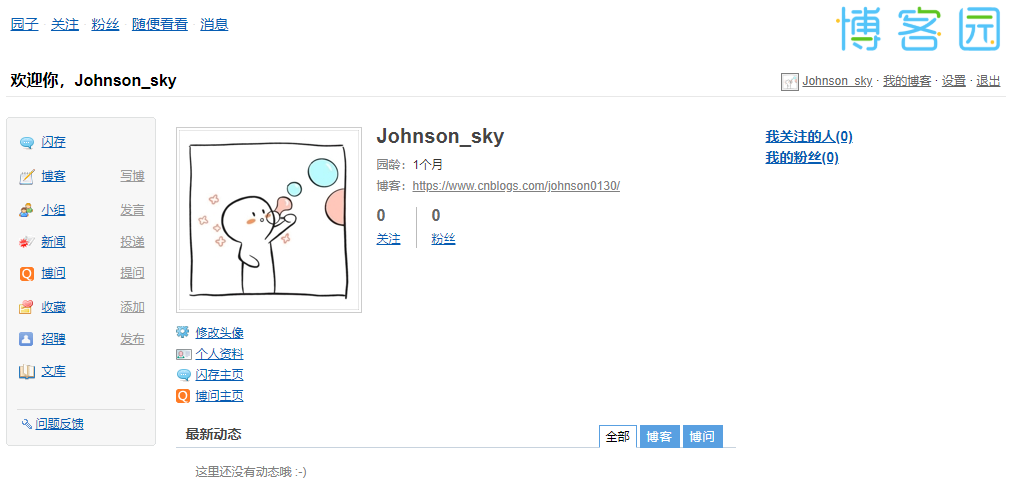
\includegraphics[scale=0.5]{F6}
    \label{fig:F6}
\end{figure}

\subsection{小木虫}

个人网址:http://muchong.com/bbs/space.php?uid=19733993

截图:
\begin{figure}[H]
    \centering
    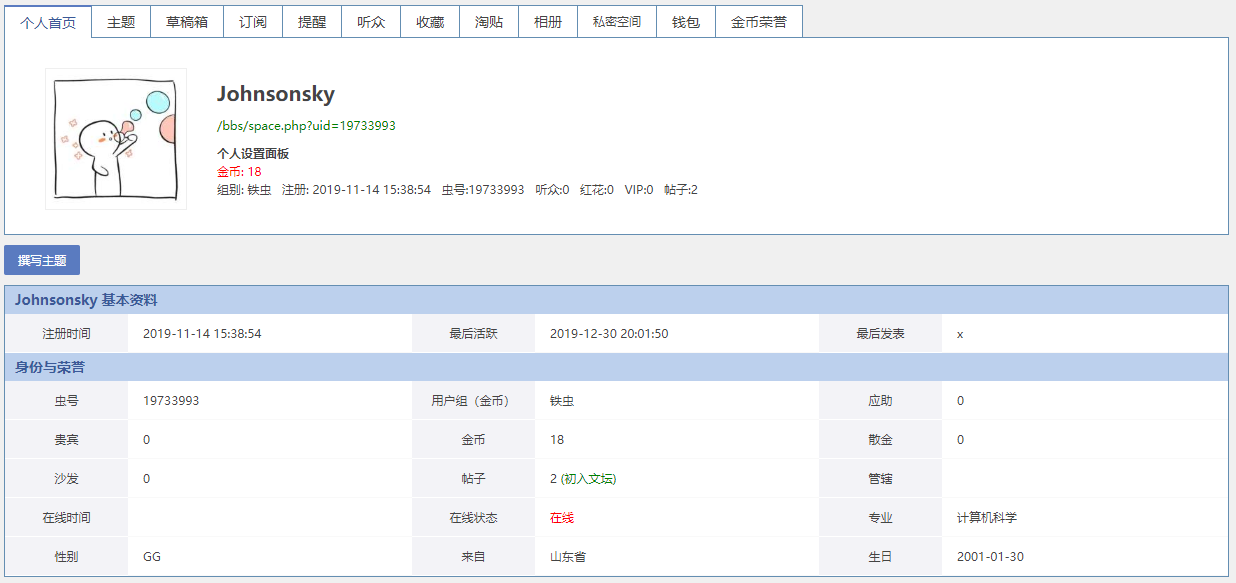
\includegraphics[scale=0.5]{F7}
    \label{fig:F7}
\end{figure}

\begin{thebibliography}{9}
    \bibitem{ref1} 杜子徳. 计算思维及其意义. 中国计算机学会通讯, 2019, 10
    \bibitem{ref2} Seymour Papert. An Exploration in the Space of Mathematics Educations[J]. International Journal of Computers for Mathematical Learning, 1996, (1): 95-123.
    \bibitem{ref3} Jeannette M. Wing. Computational Thinking[J]. Communications of the ACM, 2006, (3): 33-35
    \bibitem{ref4} 中华人民共和国教育部. 关于深化本科教育教学改革全面提高人才培养质量的意见. [2020-1-1]. moe.gov.cn/srcsite/A08/s7056/201910/t20191011\_402759.html
    \bibitem{ref5} 中国石油大学(华东)计算机科学与技术学院. 计算机科学与技术专业-工程教育认证. [2020-1-1]. ceea.upc.edu.cn
    \bibitem{ref6} 鲍旭华, 洪海, 曹志华. 破坏之王:DDoS攻击与防范深度剖析. 北京:机械工艺出版社, 2014
    \bibitem{ref7} R. Rasti, M. Murthy, N. Weaver and V. Paxson, "Temporal Lensing and Its Application in Pulsing Denial-of-Service Attacks," 2015 IEEE Symposium on Security and Privacy, San Jose, CA, 2015, pp. 187-198.
    \bibitem{ref8} R. Vishwakarma and A. K. Jain, "A Honeypot with Machine Learning based Detection Framework for defending IoT based Botnet DDoS Attacks," 2019 3rd International Conference on Trends in Electronics and Informatics (ICOEI), Tirunelveli, India, 2019, pp. 1019-1024.
    \bibitem{ref9} 中国电信, 绿盟科技. 2019年DDoS攻击态势, 2019
\end{thebibliography}


\end{document}
